\originalchapter{8.421公开作业一至五}
所有题源为Spring 2014站点公开、原件注明Spring 2012的作业. 本章解答均为编者补写. 原题的文字背景作必要缩写, 物理条件与作答要求完整保留. Gaussian单位的原式在需要时换算到SI并注明.
\originalsection{作业一: 共振演化}
\source{Assignment 1, 第1题.}
\begin{exercise}受迫经典阻尼振子远离共振时耗散功率正比于阻尼$\gamma$, 共振时却反比于$\gamma$. 为什么减小阻尼会增加共振耗散功率?\end{exercise}
\begin{solution}设$m\ddot x+m\gamma\dot x+m\omega_0^2x=F_0\cos\omega t$. 稳态振幅平方为$F_0^2/[m^2((\omega_0^2-\omega^2)^2+\gamma^2\omega^2)]$. 平均耗散功率$\overline P=m\gamma\overline{\dot x^2}=F_0^2\gamma\omega^2/[2m((\omega_0^2-\omega^2)^2+\gamma^2\omega^2)]$. 远离共振, 振幅几乎由失谐决定; 共振时减小阻尼使稳态振幅按$1/\gamma$增大, 其平方的增加超过耗散系数的下降. 达到稳态所需时间也按$1/\gamma$增加, $\gamma=0$时不存在有限稳态, 不能直接取这个端点.
\end{solution}
\source{Assignment 1, 第2题.}
\begin{exercise}在$\ket e,\ket g$基中,$H=(\hbar/2)\bigl(\begin{smallmatrix}\omega_0&\omega_R\e^{-\ii\omega t}\\\omega_R\e^{\ii\omega t}&-\omega_0\end{smallmatrix}\bigr)$. 它对应静态加旋转磁场,$\omega_0=\gamma B_0,\omega_R=\gamma B_1$. (a) 写$a_e,a_g$运动方程; (b) 给任意初态的解; (c) 初态为$g$时验证激发概率与经典磁矩结果一致.\end{exercise}
\begin{solution}(a) $\ii\dot a_e=(\omega_0a_e+\omega_R\e^{-\ii\omega t}a_g)/2$, $\ii\dot a_g=(\omega_R\e^{\ii\omega t}a_e-\omega_0a_g)/2$. (b) 令$a_e=\e^{-\ii\omega t/2}b_e,a_g=\e^{\ii\omega t/2}b_g$, $d=\omega_0-\omega$, $Q=\sqrt{d^2+\omega_R^2}$,$C=\cos(Qt/2),S=\sin(Qt/2)$. 则
\[\begin{pmatrix}a_e(t)\\a_g(t)\end{pmatrix}=\begin{pmatrix}\e^{-\ii\omega t/2}&0\\0&\e^{\ii\omega t/2}\end{pmatrix}\begin{pmatrix}C-\ii dS/Q&-\ii\omega_RS/Q\\-\ii\omega_RS/Q&C+\ii dS/Q\end{pmatrix}\begin{pmatrix}a_e(0)\\a_g(0)\end{pmatrix}.\]
(c) $P_e=\omega_R^2\sin^2(Qt/2)/Q^2$. 经典磁矩在有效场$(\omega_R,0,d)$绕转, 原先沿$-z$的向量的$z$分量改变给同一布居概率. 本题是旋转场的精确模型, 不需要对线偏振场另作旋波近似.
\end{solution}
\source{Assignment 1, 第3题.}
\begin{exercise}写$H=(\hbar/2)(V_1\sigma_x+V_2\sigma_y+\omega_0\sigma_z)$,$\rho=(r_0I+\sum_{i=1}^3r_i\sigma_i)/2$. 由von Neumann方程证明$\dot{\mathbf r}=\boldsymbol\omega\times\mathbf r$, $\boldsymbol\omega=(V_1,V_2,\omega_0)$, 并解释其物理意义.\end{exercise}
\begin{solution}代入$\dot\rho=-\ii[H,\rho]/\hbar$, 用Pauli对易子得$\dot r_k=\sum_{ij}\epsilon_{ijk}\omega_ir_j$. 单位阵系数$r_0=\Tr\rho$不变, $\dd|\mathbf r|^2/\dd t=2\mathbf r\cdot(\boldsymbol\omega\times\mathbf r)=0$. 因此幺正演化是Bloch向量的进动; 不改变纯度, 与磁矩的经典进动有相同几何.
\end{solution}

\originalsection{作业二: 原子尺度与氦}
\source{Assignment 2, 第1题.}
\begin{exercise}Gaussian单位定义$E_A=e/a_0^2$. (a) 用束缚势能和量子局域动能平衡求$a_0$量级; (b) 经典电子轨道在质子处的磁场$B_N$; (c) 与Bohr磁子作用能为一Hartree的磁场$B_H$; (d) 用$E_A$表达; (e) 哪一种更适合作原子磁场单位? 忽略无关的2因子.\end{exercise}
\begin{solution}(a) $\hbar^2/(ma_0^2)\sim e^2/a_0$, 故$a_0\sim\hbar^2/(me^2)$. (b) $v\sim\hbar/(ma_0)=\alpha c$, 移动电荷的磁场$B_N\sim(v/c)E_A=\alpha E_A$. (c) $\mu_B=e\hbar/(2mc)$,$E_h=e^2/a_0$, 所以$B_H=E_h/\mu_B\sim E_A/\alpha$. (d) 两磁场相差约$\alpha^{-2}$. (e) $B_N$描述原子内部电流自然产生的场, $B_H$描述让Zeeman能达到电子束缚能的外场. “更自然”取决于目标; 原子单位惯用$\hbar/(ea_0^2)$作磁场单位, 与$B_H$同阶. 这不否认核处内部磁场更小.
\end{solution}
\source{Assignment 2, 第2题. 原件长段文献与Feynman引文不复制.}
\begin{exercise}(a) 用Rydberg频率$f_\infty=cR_\infty$与电子静质量频率$m_ec^2/h$表达$\alpha$, 说明只需$R_\infty,h/m_e$及SI定义的$c$; (b) 用中子速度与de Broglie波长测$h/m$; (c) 用吸收频率$\nu$光子后的反冲速度测$h/m$; (d) 原子束与两束反向激光垂直相交, 第一束吸收、第二束受激退激发, 用共振频率$\nu_1,\nu_2$求反冲速度和$h/m$; (e) 用两核能级质量差$\Delta m$与发射$\gamma$波长$\lambda$求$h/\Delta m$.\end{exercise}
\begin{solution}(a) 氢的无限核质量结合能$hcR_\infty=\alpha^2m_ec^2/2$, 故$\alpha^2=2R_\infty(h/m_e)/c$. 原题的“最精确实验”叙述属于2012背景, 不在此作为当前排名. (b) $h/m=v\lambda_{\rm dB}$. (c) 动量守恒$mv_R=h\nu/c$, 故$h/m=cv_R/\nu$. (d) 忽略光子对原子静质量的极小相对修正, 横向初速零. 吸收后动量$h\nu_1/c$; 向反方向受激发射后动量$h(\nu_1+\nu_2)/c$. 两次能量守恒相减得$h(\nu_1-\nu_2)=h^2(\nu_1+\nu_2)^2/(2mc^2)$, 所以$h/m=2c^2(\nu_1-\nu_2)/(\nu_1+\nu_2)^2$, $v_R(\nu_1)=2c\nu_1(\nu_1-\nu_2)/(\nu_1+\nu_2)^2$. 近等频时$v_R\simeq c(\nu_1-\nu_2)/(2\nu)$. (e) 忽略或修正核反冲后,$\Delta mc^2=hc/\lambda$, 故$h/\Delta m=c\lambda$; 要作精密质量能量检验必须计入反冲.
\end{solution}
\source{Assignment 2, 第3题.}
\begin{exercise}氦$Z=2$, 忽略电子间作用的能量为$-108.848$ eV, 实测$-79.006$ eV. (a) 两电子均用氢样$1s$轨道并配反对称自旋, 算电子斥能及总能; (b) 改用$\phi_{Z'}=(Z'/a_0)^{3/2}\e^{-Z'r/a_0}/\sqrt\pi$, 求总能量并解释$Z'$; (c) 优化$Z'$与能量.\end{exercise}
\begin{solution}第2章的径向积分给$\langle1/r_{12}\rangle=5Z/(8a_0)$. (a) 斥能$5ZE_h/8=1.25E_h\simeq34.0$ eV, 总能$-2.75E_h\simeq-74.8$ eV. (b) $E/E_h=Z'^2-4Z'+5Z'/8$. $Z'$表示另一电子屏蔽核吸引的有效电荷, 不是真正改变核电荷. (c) $Z'=27/16$, $E=-729E_h/256\simeq-77.49$ eV. 乘积变分缺少电子坐标关联, 所以仍高于真实基态能量.
\end{solution}

\originalsection{作业三: 核大小与Breit--Rabi}
\source{Assignment 3, 第1题.}
\begin{exercise}质子视为半径$r_p=0.9$ fm的均匀带电球. (a) 求球内外势; (b) 一阶微扰求氢$1S$能移; (c) $1S\!\to2S$谱要把$r_p$测到$0.010$ fm, 所需绝对与相对频率精度是多少? 原题给$a_0=5.3\times10^{-11}$ m, Hartree的一半为13.606 eV.\end{exercise}
\begin{solution}(a) 球内$E(r)=er/(4\pi\epsilon_0r_p^3)$, 势$\phi=e(3-r^2/r_p^2)/(8\pi\epsilon_0r_p)$; 球外$\phi=e/(4\pi\epsilon_0r)$. 电子势能为$-e\phi$. (b) 球内与点核之差为$\delta V=e^2[1/r-3/(2r_p)+r^2/(2r_p^3)]/(4\pi\epsilon_0)$, 球外为零. 因$r_p\ll a_0$, 用$|\psi_{1S}(0)|^2=1/(\pi a_0^3)$, 积分得$\Delta E_{1S}=2E_h r_p^2/(5a_0^2)$, 约$3.14\times10^{-9}$ eV, 约$0.76$ MHz. (c) $2S$密度为$1S$的$1/8$, 跃迁频移为$-7\Delta E_{1S}/(8h)$. 对半径线性化误差$\delta\nu=(7/8)(2\Delta E_{1S}/h)(\delta r_p/r_p)$, 约$1.48\times10^4$ Hz. 除以$1S\!\to2S$约$2.47\times10^{15}$ Hz, 相对要求约$6.0\times10^{-12}$. 均匀球的$r_p$是外半径, rms半径为$\sqrt{3/5}r_p$, 不应把二者混用.
\end{solution}
\source{Assignment 3, 第2题.}
\begin{exercise}原题$H=ah\mathbf I\cdot\mathbf J/\hbar^2+(g_J\mu_Bm_J-g_I\mu_Bm_I)B$, $J=1/2$. (a) 推导Breit--Rabi式, $F^+=I+1/2$, $x=(g_I+g_J)\mu_BB/(ahF^+)$; (b) 对$I=3/2$画能级, 标低、高场量子数并伸到核Zeeman也可见的高场; 可用$^{87}$Rb,$g_I=0.0009954,g_J=2.002331$; (c) 列$\Delta m=0,\pm1$磁偶极跃迁的一阶不敏感点; (d) 指出哪些连接两个可磁俘获态; (e) 求$F=1,m=-1\leftrightarrow F=2,m=1$的二光子钟场, $2a=6.835$ GHz; (f) $1\,\mu$K样品经历30 mG场范围, 求该跃迁在零场和钟场的非均匀宽度.\end{exercise}
\begin{solution}(a) 第3章的二乘二推导令$A=ah$, 并把本卷带符号核因子替成$-g_I$, 得
\[E_m^\pm=-ah/4-mg_I\mu_BB\pm(ahF^+/2)\sqrt{1+2mx/F^++x^2}.\]
(b) $I=3/2$时$m=-1,0,1$各有两支, 弱场$+$为$F=2$,$-$为$F=1$. 强正场$+$为$m_J=1/2,m_I=m-1/2$,$-$为$m_J=-1/2,m_I=m+1/2$. $m=\pm2$仅有$F=2$伸展态. 记$c=g_I/(g_I+g_J)$,$\mathcal E=E/(2ah)$, 中间支$\mathcal E=-1/8-cmx\pm\sqrt{1+mx+x^2}/2$, 外支$\mathcal E_{\pm2}=3/8\pm(1/2-2c)x$. 极高场必须保留$-cmx$, 当$x\gg g_J/g_I\simeq2012$时核项的相对影响可见.

\begin{center}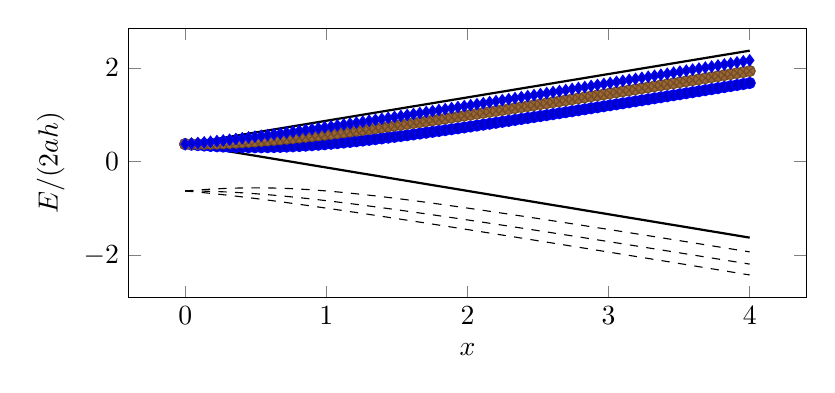
\begin{tikzpicture}\begin{axis}[width=.84\linewidth,height=5cm,xlabel={$x$},ylabel={$E/(2ah)$},domain=0:4,samples=90]
\foreach \m in {-1,0,1}{\addplot {-.125-.0004968736*\m*x+.5*sqrt(1+\m*x+x*x)};\addplot[dashed] {-.125-.0004968736*\m*x-.5*sqrt(1+\m*x+x*x)};}
\addplot[thick]{.375+.4990062528*x};\addplot[thick]{.375-.4990062528*x};
\end{axis}\end{tikzpicture}\end{center}
图示反交叉区; 极高场量子数与斜率由上面的解析渐近式给出, 避免把核尺度挤在同一张图中.

(c) 求导公式$\mathcal E_m'=-cm\pm(x+m/2)/(2\sqrt{1+mx+x^2})$, 将每一对允许$m$的斜率设相等. 正场有限根如下; 符号表示弱场支标签, 外支写$m=\pm2$:
\begin{center}\begin{tabular}{lll}\toprule
两态 & $x$ & 共同斜率$\mathcal E'$\\\midrule
$(-1,-),(-1,+)$&0.500000&0.000497\\
$(-1,-),(0,-)$&4.301496, 8.810653&$-0.487013,-0.496810$\\
$(-1,-),(0,+)$&0.268461&0.129640\\
$(-1,-),(-2)$&19.911263&$-0.499006$\\
$(-1,+),(0,-)$&0.267437&$-0.129179$\\
$(-1,+),(0,+)$&3.441655&0.480143\\
$(0,+),(1,+)$&12.379266&0.498377\\
$(1,+),(2)$&18.911263&0.499006\\\bottomrule
\end{tabular}\end{center}
另有$(0,-)\leftrightarrow(0,+)$的$x=0$钟点. 负场结果由$m\mapsto-m$获得. (d) 两态的共同斜率为正者均为低场寻求态, 即表中第1、3、6、7、8行; 零场$m=0$需看二阶曲率, 两支曲率相反, 不能一起稳定俘获. (e) 对$m=-1,-$与$m=1,+$设导数差零, 得$x=0.001324996$, $B=3.2299$ G. 这是$\Delta m=2$双光子跃迁, 不在(c)的单光子名单里. (f) 零场斜率差为$2g_I\mu_B/h$, 30 mG给约83.6 Hz. 钟点二阶系数约431 Hz/G$^2$, 若整个30 mG偏离从钟点向一侧延伸, 宽度约0.388 Hz; 若30 mG是以钟点对称的总范围, 最大偏离15 mG, 则约0.097 Hz. 原题未指定场分布, 因而必须区分这两个宽度约定.
\end{solution}
\source{Assignment 3, 第3题.}
\begin{exercise}求Na,$I=3/2$的$^2P_{1/2}$($F=1,2$)、$^2P_{3/2}$($F=0,1,2,3$)、$^2S_{1/2}$($F=1,2$)的$g$因子. 可否不用Landé公式求$P_{3/2},F=3$和$S_{1/2},F=2$伸展态?\end{exercise}
\begin{solution}忽略原题未给的核磁矩和电子异常磁矩,$g_J$分别为$2/3,4/3,2$. 再向$F$投影得$P_{1/2}$的$g_F=-1/6,1/6$;$P_{3/2}$的$F=1,2,3$均为$2/3$, $F=0$无一阶磁矩, 其Landé商式不能以$0/0$代入; $S_{1/2}$为$-1/2,1/2$. 伸展态是$m_I=I,m_J=J$的直积, 磁矩$g_JJ\mu_B$, 除以$F=I+J$即给$2/3$与$1/2$.
\end{solution}

\originalsection{作业四: 偶极与Stark淬灭}
\source{Assignment 4, 第1题.}
\begin{exercise}HCl的体轴永久电偶极为$0.41ea_0$. (a) 电磁哈密顿量在实验室转动不变, 与可测偶极有何联系? (b) 在某实验区间可测近似与场无关的偶极即线性Stark作用, 其来源是什么? (c) 为什么原子可有永久磁偶极而在保持宇称的电磁作用下没有永久电偶极?\end{exercise}
\begin{solution}(a) 零场定角动量定宇称转动态没有定向, 实验室电偶极平均为零; 体轴电荷分离并未因此消失. (b) 外场混合相反宇称的转动态, 在$d_0E$超过相关转动间隔时定向趋饱和,$\Delta E\simeq-d_0E$, 同时要求远低于电子结构变化的场尺度. (c) 空间反演使电偶极反号, 对宇称本征态其平均必须零. 磁偶极由角动量产生, 是反演不变的轴矢量, 可沿$\mathbf J$有非零平均. 永久原子EDM涉及额外对称性破缺, 不能借分子体轴偶极证明普通原子也应有EDM.
\end{solution}
\source{Assignment 4, 第2题.}
\begin{exercise}(a) 用主要$2S_{1/2},2P_{1/2}$两态模型求氢$n=2$的Stark能量和态, 解释忽略$2P_{3/2}$的条件; 细结构间隔约10 GHz,Lamb间隔1.06 GHz, 题给偶极$3ea_0$. 线性区所需场量级及MHz/(V/cm)斜率是多少? (b) 初态$2S=a$, 衰减$\Gamma_a=8$ s$^{-1}$,$2P=b$衰减$\Gamma_b=6.3\times10^8$ s$^{-1}$. 耦合为$\hbar V$, 相隔$\hbar\omega_0$. 解$a(t)$并讨论强弱耦合和能移. (c) 求淬灭寿命$1\,\mu$s的场, 分别忽略Lamb间隔和保留实际间隔, 用弱场近似.\end{exercise}
\begin{solution}(a) 两态能量$\pm\hbar\sqrt{\omega_0^2+4|V|^2}/2$, $V=dE/\hbar$. 混合角$\tan2\theta=2|V|/\omega_0$, 本征态为$\cos\theta\ket a+\sin\theta\ket b$及其正交组合, 相位按$V$符号选定. $d/h=3ea_0/h$给3.84 MHz/(V/cm), 强混合边界约138 V/cm; 充分线性需更大但仍使$dE/h\ll10$ GHz以压低$P_{3/2}$混合. 题给$3ea_0$为其简化模型参数, 不另声称已做完整精细结构CG投影.

(b) 令$\widetilde b=\e^{\ii\omega_0t}b$, 则$\dot a=-\Gamma_a a/2-\ii V^*\widetilde b$,$\dot{\widetilde b}=-(\Gamma_b/2-\ii\omega_0)\widetilde b-\ii Va$. 记$q=\Gamma_b/2-\ii\omega_0$, 先忽略$\Gamma_a$, 两指数根$\mu_{1,2}=[q\pm\sqrt{q^2-4|V|^2}]/2$. 由$a(0)=1,\dot a(0)=0$得$a(t)=[\mu_1\e^{-\mu_2t}-\mu_2\e^{-\mu_1t}]/(\mu_1-\mu_2)$. 弱场慢根$\mu_s\simeq|V|^2/q$, 布居衰减率
\[\Gamma_{\rm eff}\simeq\Gamma_a+\frac{|V|^2\Gamma_b}{\omega_0^2+(\Gamma_b/2)^2}.\]
虚部给$2S$向上能移$\hbar|V|^2\omega_0/[\omega_0^2+(\Gamma_b/2)^2]$, 远大于线宽时恢复微扰Stark位移. 强耦合$|V|\gg\omega_0,\Gamma_b$有快速两态振荡, 两本征态约各含一半$P$, 布居包络衰减率约$\Gamma_b/2$.

(c) 取$\Gamma_{\rm eff}=10^6$ s$^{-1}$. 忽略间隔时$|V|=\sqrt{\Gamma_{\rm eff}\Gamma_b}/2=1.255\times10^7$ s$^{-1}$, 场约0.520 V/cm. 保留$\omega_0=2\pi\times1.06$ GHz时,$|V|=\sqrt{\Gamma_{\rm eff}[\omega_0^2+(\Gamma_b/2)^2]/\Gamma_b}=2.656\times10^8$ s$^{-1}$, 场约11.0 V/cm. Lamb位移抑制混合, 因而要求约21倍更强的场.
\end{solution}

\originalsection{作业五: 光阱与差分光移}
\source{Assignment 5, 第1题.}
\begin{exercise}碱金属基态的振子强度近乎集中在$S\to P$频率$\omega_0$. 用强度$I$, 红失谐$\omega_L<\omega_0$驱动. (a) 分别求含反旋项和旋波弱场的AC位移, 比较其比值在共振附近和$\omega_L\to0$的极限; (b) 求两模型的时均激发态概率; (c) 用振荡偶极辐射功率求散射率, 比较$\Gamma P_e$并解释虚态图; (d) Na,$\lambda_0=590$ nm, Gaussian光束$I(r)=2P\e^{-2r^2/w^2}/(\pi w^2)$,$w=6\,\mu$m, 势深$k_B\times10\,\mu$K. 比较红失谐1.7 GHz黄光与985 nm红外光所需功率和散射率, 哪个更适合旋波近似?\end{exercise}
\begin{solution}记$d$为等效跃迁偶极, $C=d^2E_0^2/(4\hbar)$,$\Delta=\omega_L-\omega_0$,$I=\epsilon_0cE_0^2/2$. (a) $U_i=-C[1/(\omega_0-\omega_L)+1/(\omega_0+\omega_L)]$, $U_{ii}=C/\Delta$. 比值$2\omega_0/(\omega_0+\omega_L)$, 共振近1, 很慢交流场的周期平均极限为2. 直接设$\omega_L=0$的恒定DC场不再平均$\cos^2$, 实际静态位移是这里交流极限的两倍. (b) 这里指场绝热打开、瞬态消失后的周期响应, 不是$t=0$突然打开且初态为裸基态的无衰减问题. 一阶激发幅度含两个稳态分量, 两分母为$\omega_0-\omega_L$和$\omega_0+\omega_L$, 在非零$\omega_L$下平均过足够多周期后
\[P_{e,i}=\frac{d^2E_0^2}{4\hbar^2}\left[\frac1{(\omega_0-\omega_L)^2}+\frac1{(\omega_0+\omega_L)^2}\right],\quad P_{e,ii}=\frac{d^2E_0^2}{4\hbar^2\Delta^2}.\]

若从裸基态突然打开无衰减场, 还会有自由瞬态. 令$A=(\omega_0-\omega_L)^{-1},B=(\omega_0+\omega_L)^{-1}$, 一阶Schrödinger幅度（整体符号无关）为
\[c_e(t)=\frac{dE_0}{2\hbar}
 [A\e^{-\ii\omega_Lt}+B\e^{\ii\omega_Lt}-(A+B)\e^{-\ii\omega_0t}].\]
在非零、非共振频率下长时间平均为$d^2E_0^2(A^2+B^2+AB)/(2\hbar^2)$, RWA突然打开则为$d^2E_0^2/(2\hbar^2\Delta^2)$, 与已建立周期响应相差瞬态贡献. 题面未给打开方式时须先约定, 散射稳态使用前述周期响应而不是这个无衰减瞬态平均.

(c) $d_{\rm ind}=\alpha_iE_0$, $R_i=\omega_L^3|\alpha_iE_0|^2/(12\pi\epsilon_0\hbar c^3)$, 其中$\alpha_i=2d^2\omega_0/[\hbar(\omega_0^2-\omega_L^2)]$. 用$\alpha_{ii}=d^2/[\hbar(\omega_0-\omega_L)]$定义对应旋波散射结果, 得$R_{ii}=\Gamma P_{e,ii}(\omega_L/\omega_0)^3$, $R_i/R_{ii}=[2\omega_0/(\omega_0+\omega_L)]^2$. 因两振幅相干, 全模型一般不等于$\Gamma P_{e,i}$乘单一因子. 虚态高度为$\hbar\omega_L$, 发射光频也为$\omega_L$, 有效辐射率相对自然率含$(\omega_L/\omega_0)^3$; 若仅按旋波单路径的$R_{ii}=\Gamma P_{e,ii}(\omega_L/\omega_0)^3$定义形式上的辐射等待时间, 可写$\tau_{\rm virt}^{(ii)}=P_{e,ii}/R_{ii}=\Gamma^{-1}(\omega_0/\omega_L)^3$. 这是原(c)(iii)所用虚寿命类比的条件化版本, 全含反旋项的两路径相干散射一般不能以同一比例解释. 虚能量标记并非可独立占据并有普通寿命的真正能级.


\begin{center}\begin{tikzpicture}[>=Stealth,x=1cm,y=1cm]
\draw[thick](0,0)--(3.8,0) node[right]{$S$};
\draw[thick](0,2.4)--(3.8,2.4) node[right]{$P,\ \hbar\omega_0$};
\draw[dashed](.2,1.45)--(3.8,1.45) node[right]{$\hbar\omega_L$虚能量标记};
\draw[->,blue,thick](.8,.06)--(.8,1.4) node[midway,left]{$\omega_L$};
\draw[->,red,thick](2.6,1.4)--(2.6,.06) node[midway,right]{$\omega_L$};
\node[align=center] at(1.8,-.65){吸收与发射同频; 虚标记不是真正原子能级};
\end{tikzpicture}\end{center}

(d) 用$f\simeq1$等效模型,$d^2=\hbar e^2/(2m_e\omega_0)$, 及$\Gamma=\omega_0^3d^2/(3\pi\epsilon_0\hbar c^3)$完成计算. 黄光$P\simeq1.00\times10^{-7}$ W,$R\simeq7.83\times10^3$ s$^{-1}$; 红外$P\simeq9.61\times10^{-3}$ W,$R\simeq1.76\times10^{-2}$ s$^{-1}$. 这里数值采用题设单等效振子, 真实Na的D线多重态可改变常数. 黄光的$|\Delta|\ll\omega_0$适合旋波, 红外应保留反旋项; 固定阱深下红外散射显著较低.
\end{solution}
\source{Assignment 5, 第2题.}
\begin{exercise}激光以频率$\omega$, 强度$I$作用于$S,P$两态, 间隔$\omega_{PS}$, 偶极$d_{PS}$, 不作旋波. (a) 求两光移及差分光移能否为零; (b) 加更高$D$态, $\omega_{PS}=f\omega_{DP},d_{PS}=nd_{DP}$, $S,D$不直接耦合, 求$P$光移和magic频率.\end{exercise}
\begin{solution}定义$F(\omega_j)=\omega_j/(\omega_j^2-\omega^2)$及$K=E_0^2/(2\hbar)$. (a) $U_S=-Kd_{PS}^2F(\omega_{PS})$,$U_P=+Kd_{PS}^2F(\omega_{PS})$. 有非零有限光阱时差分位移不可能零. (b) $U_P=K[d_{PS}^2F(\omega_{PS})-d_{DP}^2F(\omega_{DP})]$. 令$U_P=U_S$得$2n^2f/(f^2-y)=1/(1-y)$,$y=\omega^2/\omega_{DP}^2$, 所以$y=(2n^2f-f^2)/(2n^2f-1)$. 需$y>0$且避开真实共振, 方为本模型有效magic解. 原题要求“以$d_{DP}$表达”, 但偶极绝对值在等光移条件中抵消, 只剩比$n$.
\end{solution}
\source{Assignment 5, 第3题.}
\begin{exercise}碱金属$S_{1/2}$耦合$P_{1/2},P_{3/2}$, 频率$\omega_1,\omega_2$. 偶极平方: $S,+1/2\to P_{3/2},+3/2$为$d_2^2$, $S,-1/2\to P_{3/2},+1/2$为$d_2^2/3$; 反向圆偏振对应对称两项; $S,+1/2\to P_{1/2},-1/2$及$S,-1/2\to P_{1/2},+1/2$为$2d_1^2/3$. 不作旋波. (a) 沿$z$传播,$x$线偏振, 求零光移波长; Rb数据$\lambda_1=795$ nm,$\lambda_2=780$ nm,$d_1=3.0ea_0,d_2=4.2ea_0$. 与实验用790 nm是否符合, 忽略了什么? (b) $\sigma^+$且主要耦合$P_{3/2}$, 求两个自旋光移, 写成标量加虚磁场,$g_J=2$.\end{exercise}
\begin{solution}(a) 线偏振的两圆分量各占一半, 两基态均有$U=-K[d_1^2F(\omega_1)/3+2d_2^2F(\omega_2)/3]$. 零点满足$\omega^2=[d_1^2\omega_1\omega_2^2+2d_2^2\omega_2\omega_1^2]/[d_1^2\omega_1+2d_2^2\omega_2]$, 给约791.93 nm. 与790 nm相近但不相同; 题给偶极矩把实际不同$J$的径向矩阵元和角系数作了简化, 还忽略超精细、多余跃迁与偏振误差. 不能用实验值反向修改题给矩阵元使答案恰好790 nm. (b) $U_+=-Kd_2^2F_2,U_-=-Kd_2^2F_2/3$. 因而$U_S=-2Kd_2^2F_2/3$, $U_V=-2Kd_2^2F_2m_J/3$, $B_{\rm eff}=-Kd_2^2F_2/(3\mu_B)$, 符号以题给$U_V=g_Jm_J\mu_BB_{\rm eff}$约定.
\end{solution}
